\chapter{FERRAMENTAS E TECNOLOGIAS UTILIZADAS}
\label{chap:ferramentasDeDesenvolvimento}

Esse capítulo expõe as ferramentas e tecnologias que foram utilizadas para o desenvolvimento deste trabalho. Para o desenvolvimento das interfaces de usuário foi utilizado \textit{ReactJS} auxiliado por outras bibliotecas secundárias. Já para desenvolver a API \textit{back-end} foi aplicado o padrão REST através do \textit{framework NestJS}. Por fim, conectado a tudo isso, o gerenciador de banco de dados \textit{PostgreSQL} foi empregado. Nos próximos sub-capítulos tais tecnologias (e outras que também estão envolvidas) serão melhor pormenorizadas.

\section{JavaScript}
\label{sec:javascript}
JavaScript é uma linguagem de programação adotada amplamente pela maioria das páginas \textit{web}, além de ser utilizada também em outros ambientes fora do navegador através de tecnologias auxiliares. Trata-se de uma linguagem interpretada, originalmente implementada diretamente como parte dos navegadores \textit{web} para que os scripts pudessem ser executados \textit{client-side} sem a necessidade de passar por um servidor \cite{Mozilla2023}.

JavaScript é baseado em protótipos, leve, dinâmico e \textit{single-thread}, dando suporte a vários paradigmas de programação diferentes, como a programação orientada a objetos, a imperativa e a declarativa. Além disso, diferencia-se também por utilizar o tipo de compilação \textit{just-in-time}, compilando seu código durante a sua execução \cite{Mozilla2023}.

\image
    {Código exemplo em JavaScript}
    {javascript}
    {data/figures/javascript.png}
    {width=.65\textwidth}
    {Autor}

A linguagem foi criada em 1995 pelo programador Brendan Eich e sua equipe a pedido da empresa NetScape para lidar com a validação de formulários HTML. Para que a linguagem evoluísse obedecendo padronizações já estabelecidas no mercado, os criadores da linguagem associaram-se à fundação ECMA um ano após sua criação, entretanto, o nome JavaScript já havia sido patenteado, decidindo-se seguir pelo nome oficial de ECMAScript \cite{Malavasi2017}.

Todavia, de acordo com \citeonline{Malavasi2017}, na comunidade de desenvolvedores a linguagem ainda é chamada de JavaScript até os dias atuais, utilizando o nome oficial ECMAScript apenas para referenciar suas versões.
\section{TypeScript}
\label{sec:typescript}
TypeScript é uma linguagem de programação desenvolvida pela Microsoft em 2012 de código aberto. Por definição, consiste-se de um superconjunto do JavaScript, adicionando também tipagem estática a linguagem original \cite{Microsoft2023}.

Por tratar-se de superconjunto, tudo o que existe em sua linguagem “mãe” também está presente nesta linguagem, incrementada pelas novas suas funcionalidades, como por exemplo: tipos, orientação à objetos, \textit{decorators}, \textit{mixins}, módulos e \textit{namespaces} \cite{Goldberg2022}.Além disso, essa peculiaridade também faz com que todo código JavaScript também seja um código TypeScript minimamente válido, facilitando assim possíveis migrações de projetos.

Pela natureza do JavaScript de ser compilado \textit{just-in-time}, muitos erros frugais de desenvolvimento são percebidos apenas na hora da execução do código. Entretanto, pelo TypeScript ser estaticamente tipado, o paradigma de orientação a objetos é acentuadamente estimulado \cite{Goldberg2022}. Ao alinhar isso ao sistema de tipos da linguagem, erros de programação tornam-se evidentes muito brevemente, conforme exemplifica a  figura a seguir:

\begin{figure}[H]
    \centering
    \caption{Comparação de códigos TypeScript e JavaScript.}
    \label{fig:typescript}
    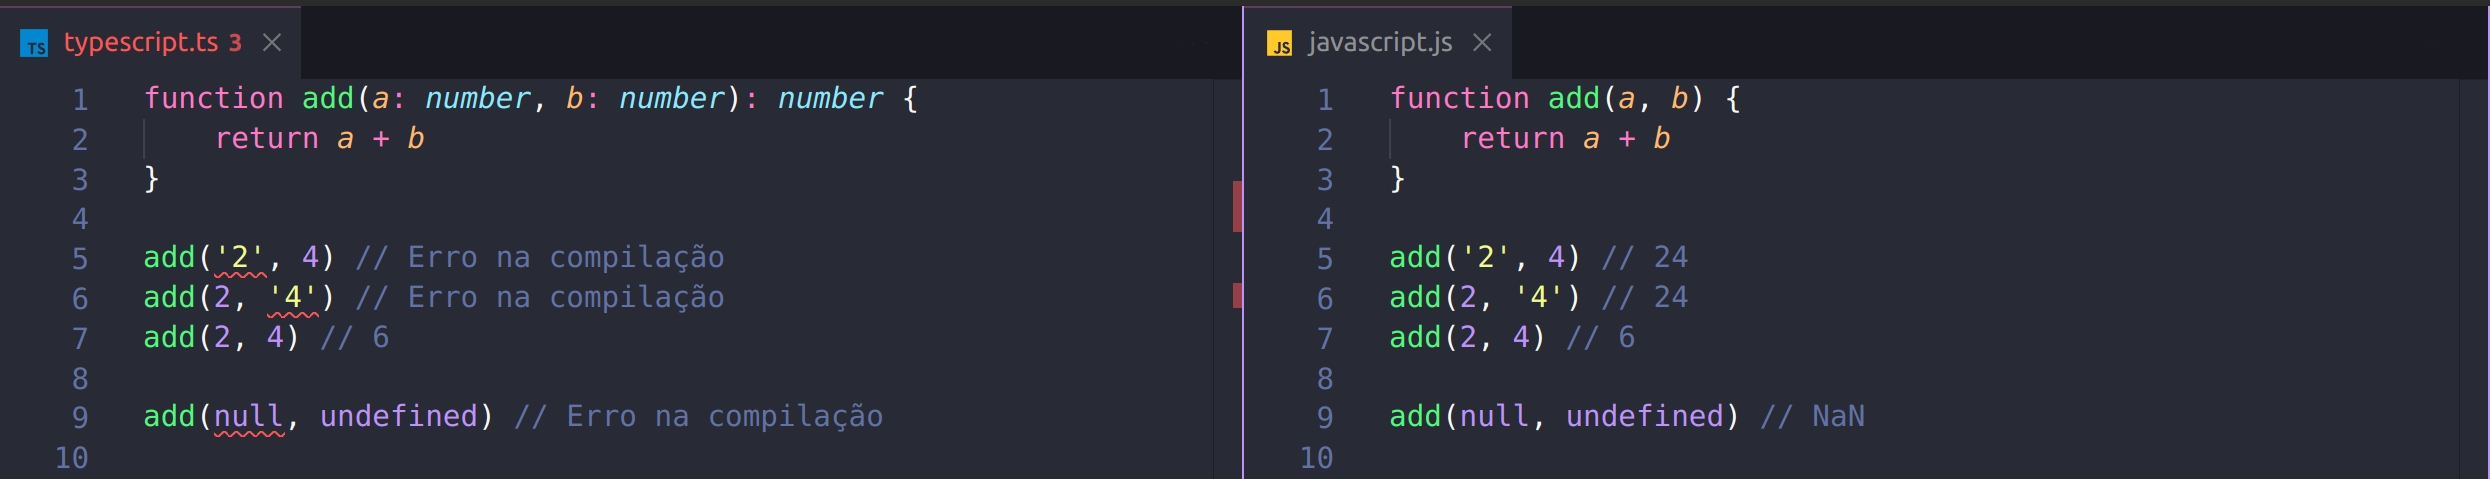
\includegraphics[width=1\textwidth]{data/figures/typescript-javascript.jpg}
    \fonte{Autor}
\end{figure}

Além de tudo, segundo \citeonline{Microsoft2023a}, a estrutura padrão do JavaScript acaba por não conseguir acompanhar o crescimento exponencial de tamanho, escopo e complexidade de suas novas aplicações, reduzindo a capacidade de escalabilidade da linguagem, problemática que é profundamente saciada pelas funcionalidades extras do TypeScript.

Por fim, pelos navegadores efetivamente darem suporte exclusivamente a códigos JavaScript, o TypeScript necessita ser pré-processado antes de ser empregado no \textit{client-side}, tornando sua linguagem “mãe” imprescindível à sua construção. Seu compilador padrão é o tsc, e outros agregadores mantidos pela comunidade (como o esbuild e o babel) podem ser utilizados a partir da necessidade específica de cada projeto \cite{Microsoft2023a}.


\section{NodeJS}
\label{sec:nodejs}
NodeJS é um ambiente de execução de código JavaScript e TypeScript externo a um navegador \textit{web}. Este software inspira-se por sistemas como a máquina de eventos da linguagem Ruby e o Twist do Python para caracterizar-se pela sua arquitetura assíncrona e orientada por eventos \cite{Foundation2023}. 

Sua implementação é contrastante em relação à outras tecnologias pois não apresenta o modelo convencional de simultaneidade, onde conceitos de threads do sistema operacional são empregados.  Seu \textit{runtime} é executado por apenas uma \textit{thread} que executa o \textit{looping} de eventos, que perdura desde a criação da \textit{thread} até quando não há mais retornos de chamadas a serem concluídos \cite{Foundation2023}.

Dentro desse mesmo contexto, chamadas que normalmente seriam bloqueantes (que requerem recursos do sistema operacional) são realizadas assíncronamente utilizando a biblioteca libuv \cite{ClaudioWunder}. Na Figura 8 é possível visualizar um diagrama simplificado desse fluxo.

\begin{figure}[H]
    \centering
    \caption{\textit{Looping} de eventos NodeJS.}
    \label{fig:nodejs}
    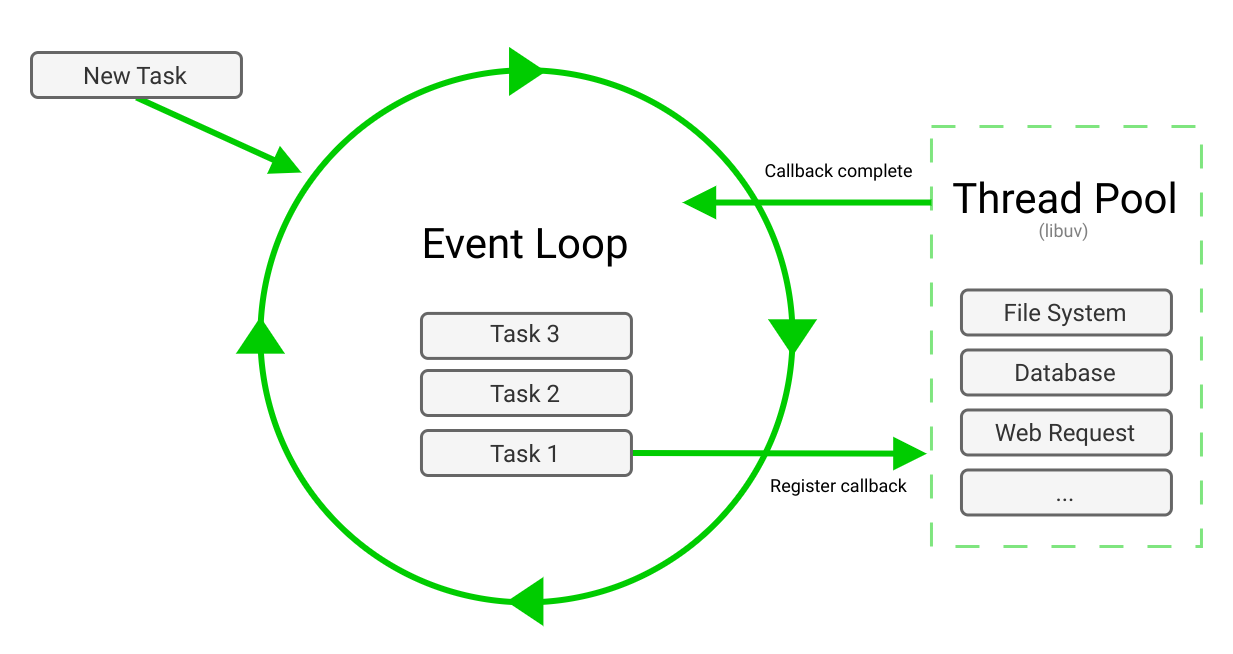
\includegraphics[width=.8\textwidth]{data/figures/nodejs.png}
    \fonte{Autor}
\end{figure}

Além disso, o NodeJS também dispõe do NPM, um gerenciador de pacotes reutilizáveis de código aberto, permitindo maior agilidade, flexibilidade e produtividade no processo de desenvolvimento \cite{npm2022}.
\section{ReactJS}
\label{sec:reactJS}
ReactJS é uma biblioteca NodeJS de código aberto criada pelo Facebook em 2011 para o desenvolvimento de interfaces \textit{web} em JavaScript e/ou Typescript. Comparando-o com outras bibliotecas e \textit{frameworks} para o desenvolvimento \textit{web front-end}, constata-se que seu diferencial se encontra na abordagem de construção da interface baseada em componentes atualizados e sincronizados de forma muito mais otimizada \cite{Source2023}.

A arquitetura base de um projeto ReactJS consiste em uma estrutura hierárquica de componentes onde cada componente representa uma parte da interface final do usuário, que possui sua própria lógica e aparência isolada de outros componentes. Nesse contexto, um dos caminhos ideais da construção do código encontra-se no princípio de “separação de conceitos”, onde cada seção (ou componente) é responsável por lidar com apenas um assunto separadamente e nada além disso, resultando em uma arquitetura mais modular e escalável \cite{Qawwas2022}.

Empiricamente, cada componente React é uma função que retorna uma pequena porção de código HTML, que é estilizado por código CSS e passível de ser modificado pelas lógicas em JavaScript/TypeScript que existem dentro dessa mesma função, permitindo assim que esse pedaço de interface usufrua de todas funcionalidades que essas linguagens de programação oferecem \cite{Qawwas2022}.

\begin{figure}[H]
    \centering
    \caption{Código exemplo em ReactJS.}
    \label{fig:reactJS}
    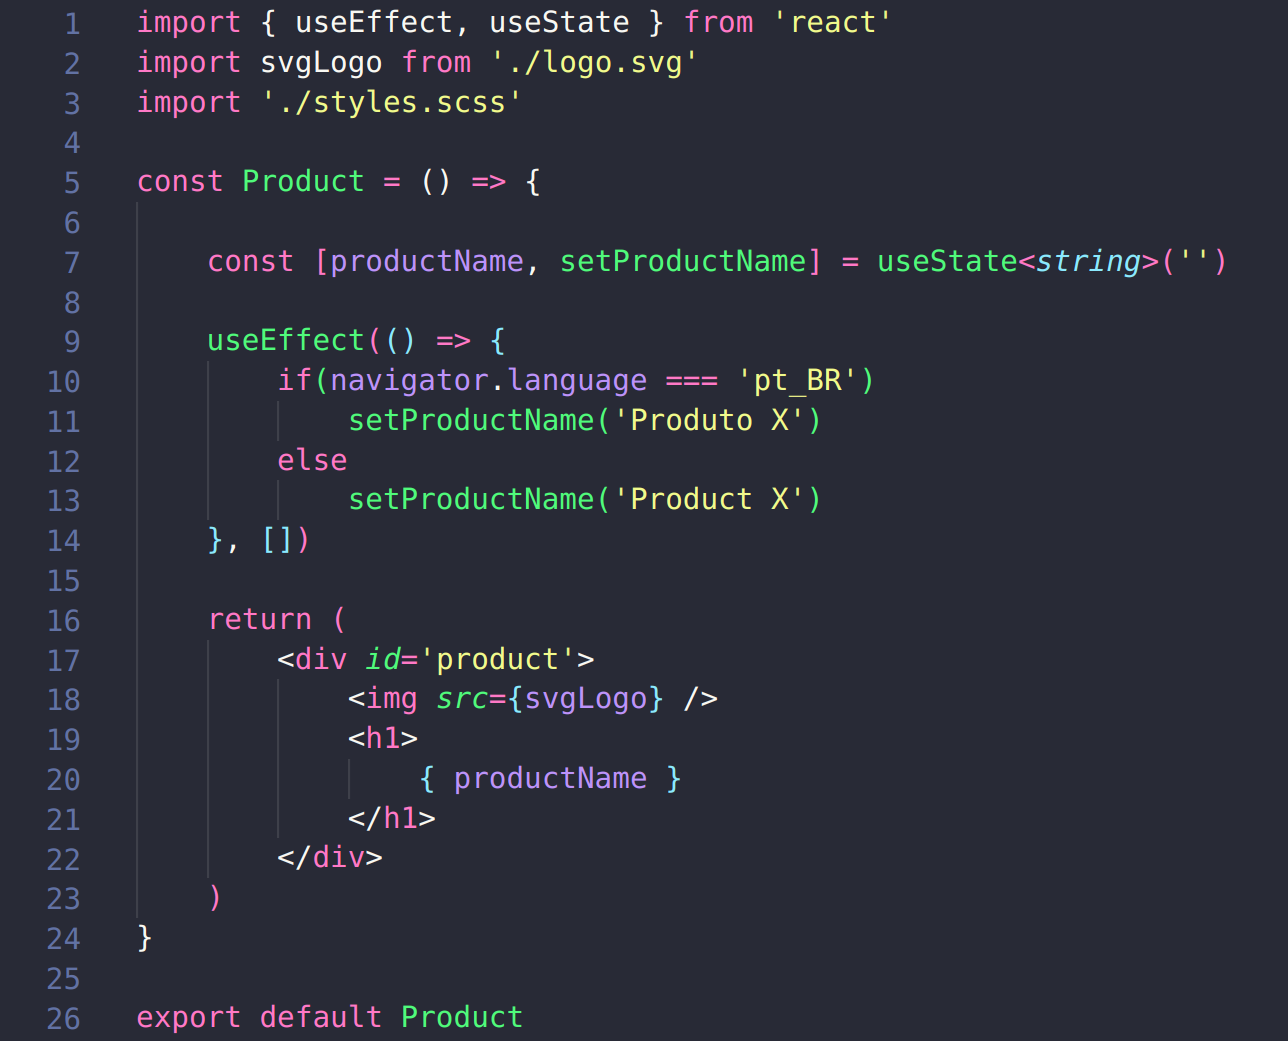
\includegraphics[width=.7\textwidth]{data/figures/react.png}
    \fonte{Autor}
\end{figure}

Atualmente, de acordo com a pesquisa Developer Survey realizada pela \citeonline{Exchange2023}, ReactJS é a biblioteca de desenvolvimento \textit{web} mais utilizada no âmbito profissional, refletindo o amplo apoio que a biblioteca possui em novas funcionalidades e resolução de problemas.
\section{NestJS}
\label{sec:nestjs}
NestJS é um framework em NodeJS de código aberto lançado em 2017 para o desenvolvimento de aplicações \textit{server-side}. Diante de outras tecnologias já consolidadas no JavaScript, esse \textit{framework} destaca-se por sua implementação base sustentar-se em elementos de programação orientada a objetos, programação funcional e programação reativa funcional para prover maior eficiência e escalabilidade \cite{Mysliwiec2023b}.

Arquiteturalmente, para ser uma \textit{API RESTful} e aplicar o protocolo HTTPS, o NestJS não reinventa a roda e por baixo dos panos utiliza outros \textit{frameworks} consagrados no mercado, como o ExpressJS e Fastify, deixando a encargo do desenvolvedor decidir qual irá ser utilizado. Ao fazer isso, essa tecnologia também permite a utilização da ampla gama de bibliotecas auxiliares do NodeJS, adaptando-se facilmente às peculiaridades de cada projeto \cite{Mysliwiec2023}.

Além disso, de acordo com a comunidade, à nível de organização de código, NestJS inspira-se fortemente no framework \textit{front-end} Angular \cite{Passos2018}. Partindo disso, uma aplicação NestJS consiste em uma organização hierárquica de múltiplos módulos onde cada módulo é encarregado de um fragmento da aplicação, possuindo seus componentes, \textit{middlewares}, filtros, \textit{pipes} e protetores de rota.

Por fim, a tecnologia dispõe de sua própria interface de linha de comando, onde é possível inicializar a estrutura base do projeto além de também incluir de maneira simplificada novos módulos à aplicação \cite{Mysliwiec2023a}.

\begin{figure}[H]
    \centering
    \caption{Estrutura base de um projeto NestJS.}
    \label{fig:nestjs}
    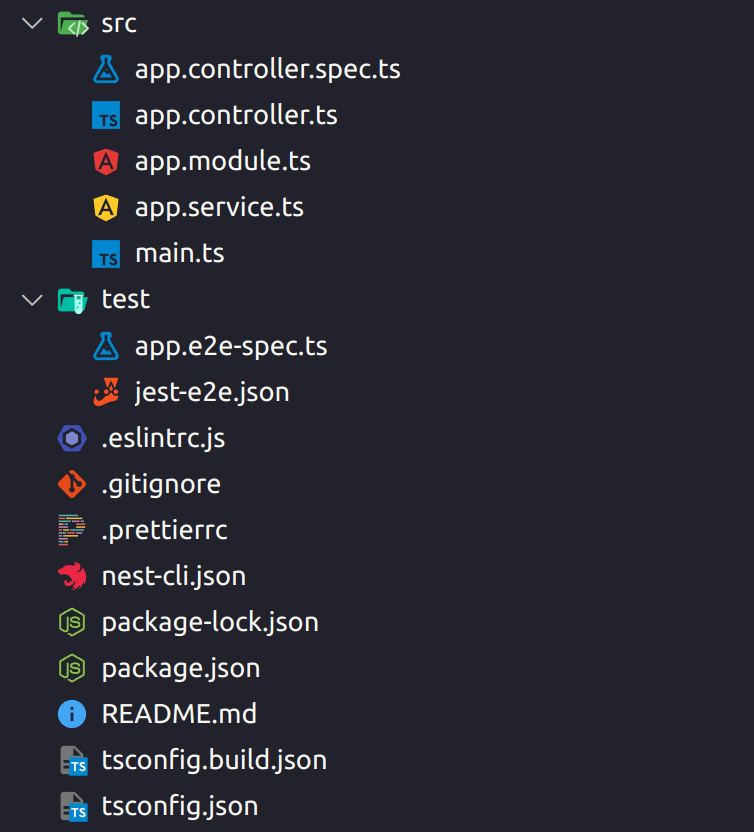
\includegraphics[width=.4\textwidth]{data/figures/nest.png}
    \fonte{Autor}
\end{figure}
\section{PostgreSQL}
\label{sec:postgresql}
PostgreSQL	trata-se de um sistema gerenciador de banco de dados de código aberto, muito famoso e utilizado amplamente no âmbito empresarial. Esse sistema caracteriza-se principalmente por sua arquitetura robusta, fácil instalação, uso prático e possibilidade de utilização de extensões \cite{PostgreSQL2023}.

\begin{citacao}
    "O PostgreSQL conquistou uma forte reputação por sua arquitetura comprovada, confiabilidade, integridade de dados, conjunto robusto de recursos, extensibilidade e a dedicação da comunidade de código aberto por trás do software para fornecer consistentemente soluções inovadoras e de alto desempenho. O PostgreSQL é executado em todos os principais sistemas operacionais , é compatível com ACID desde 2001 e possui complementos poderosos, como o popular extensor de banco de dados geoespacial PostGIS."

    \citeonline{PostgreSQL2023}.
\end{citacao}

Em respeito a sua arquitetura, PostgreSQL estrutura-se de maneira simplória, possuindo uma memória compartilhada, processos de \textit{background} e sistema de diretório de dados. Em um fluxo usual, o cliente realiza uma solicitação ao servidor, que então processa os dados utilizando buffers compartilhados e processos em segundo plano \cite{Kinsta2023}.
